\documentclass[12pt,a4paper]{article}
\PassOptionsToPackage{quiet}{fontspec}
% \usepackage[utf8]{inputenc} % 允许使用 UTF-8 字符编码
\usepackage[dvipsnames]{xcolor} % 颜色
\usepackage[UTF8]{ctex} % 支持中文字符
\usepackage{amsmath, amssymb, bm} % 数学公式
\usepackage{graphicx} % 插入图片
\usepackage{geometry} % 页面布局
\usepackage{listings} % 代码块
\usepackage{hyperref} % 超链接
\usepackage{booktabs} % 表格美化
\usepackage{longtable} % 长表格
\usepackage{multirow} % 多行表格
\usepackage{caption} % 图表标题
\usepackage{subcaption} % 子图
\usepackage{algorithm} % 算法环境
\usepackage{algpseudocode} % 算法伪代码
\usepackage{pgfplots} % 画图
\usepackage{tikz} % 画图工具
\usepackage{subcaption} % 子图
\usepackage[
    %backend=biber, 
    natbib=true,
    style=numeric,
    sorting=none
]{biblatex}
% \addbibresource{references.bib} % 引用文献库


\geometry{left=3cm,right=3cm,top=2.5cm,bottom=2.5cm}
\renewcommand\contentsname{目录}
\renewcommand\figurename{图}
\renewcommand\tablename{表}

% 代码块风格设置
\lstset{
    language=Python, % 假设使用 Python,如果用其他语言可以修改
    basicstyle=\linespread{0.9}\ttfamily\scriptsize,
    keywordstyle=\color{teal},
    commentstyle=\color{green!30!gray},
    stringstyle=\color{brown},
    frame=single,
    backgroundcolor = \color{gray!5},
    breaklines=true,
    captionpos=b,
    numbers=left,
    numberstyle=\tiny\color{gray},
    columns=flexible,
    showstringspaces=false
}

\title{\textbf{强化学习作业1:倒立摆/冰壶游戏}}
\date{2025年4月5日}

\begin{document}

\maketitle

\tableofcontents
\newpage


\section{内容概述}
本作业实现了两种强化学习算法(DQN和PPO)用于解决两个环境问题:倒立摆(Pendulum)控制和冰壶(Curling)游戏。在两个环境中,分别训练并评估了两种算法的效果,提出了一系列改进措施增强性能,可视化并分析结果。

第\ref{sec:env}节阐述了倒立摆和冰壶的环境搭建,以及一系列改进策略。第\ref{sec:algo}节介绍了DQN和PPO的算法核心思想及代码实现。第\ref{sec:experienment}节对两个算法在两个环境中的实验进行分析。第\ref{sec:conclusion}节对作业内容进行总结。代码的具体使用方法见\colorbox{gray!20}{\texttt{README.md}}。

\section{环境}
\label{sec:env}
\subsection{倒立摆}
环境为一个一阶倒立摆,由电机直接驱动。初始状态为摆竖直向下,角速度为0,目标状态为摆竖直向上,并稳定在最高点。离散的动力学模型为:
\begin{equation}
\ddot{\alpha} = \frac{1}{J} ( mgl \sin(\alpha) - b \dot{\alpha} - \frac{K^2}{R} \dot{\alpha} + \frac{K}{R} u )
\end{equation}
\begin{equation}
\begin{cases}
\alpha_{k+1} = \alpha_k + T_s \dot{\alpha}_k \\
\dot{\alpha}_{k+1} = \dot{\alpha}_k + T_s \ddot{\alpha}(\alpha_k, \dot{\alpha}_k, u_k)
\end{cases}
\end{equation}
对应代码:
\begin{lstlisting}
# envs/pendulum_env.py
# ...
class PendulumEnv(Env):
# ...
    def __init__(self, m, g, l, J, b, K, R, max_voltage, max_speed, Ts, max_steps):
        # ...
        self.constants = self._calculate_constants()
        # ...
# ...
    def _calculate_constants(self) -> tuple:
        """
        Calculate constants for calculation based on the parameters of the pendulum.
        """
        return (
            self.m * self.g * self.l / self.J,
            (-self.b - np.power(self.K, 2) / self.R) / self.J,
            self.K / (self.J * self.R),
        )
# ...
    def step(self, action: float) -> tuple:
        # ...
        # Calculate the new state based on the action
        self.ddot_alpha = (
            self.constants[0] * np.sin(self.alpha) + self.constants[1] * self.dot_alpha + self.constants[2] * action
        )
        self.dot_alpha += self.ddot_alpha * self.Ts
        self.alpha += self.dot_alpha * self.Ts
        # alpha is limited to [-pi, pi)
        self.alpha = ((self.alpha + np.pi) % (2 * np.pi)) - np.pi
        # dot_alpha is limited to [-max_speed, max_speed]
        self.dot_alpha = np.clip(self.dot_alpha, -self.max_speed, self.max_speed)
        self.state = (self.alpha, self.dot_alpha)
# ...
\end{lstlisting}

作业要求中给出的奖励函数为:
\begin{equation}
\mathcal{R}(s, a) = -s^T Q_{rew} s - R_{rew} a^2
\tag{4}
\end{equation}
其中,
\begin{equation}
Q_{rew} = 
\begin{bmatrix}
5 & 0 \\
0 & 0.1
\end{bmatrix}, \quad R_{rew} = 1.
\end{equation}

但在实验中发现,原始奖励函数会让模型收敛于局部最优(电机输出力矩与倒立摆重力平衡的位置)。因此,修改奖励函数如下:
\begin{equation}
\begin{cases}
    \mathcal{R}(s, a) = \mathcal{R}_{\text{base}}(s) + \mathcal{R}_{\text{extra}}(s, a),
    & \text{if } |\alpha| < 20^{\circ}
    \\
    \mathcal{R}(s, a) = \mathcal{R}_{\text{base}}(s),
    & \text{otherwise}
\end{cases}
\end{equation}
其中,
\begin{equation}
\begin{cases}
    \mathcal{R}_{\text{base}}( s ) = 0.05 \left(-|\alpha| + \frac{\pi}{2} + 0.001 e^{5(-|\alpha| + \frac{\pi}{2})}\right)
    \\
    \mathcal{R}_{\text{extra}}( s, a ) = 0.1 - 0.05 \tanh ( 0.1 \cdot |\dot{\alpha}| ) - 0.05 \tanh ( 0.1 \cdot |a| )
\end{cases}
\end{equation}

修改后的奖励与原始奖励对比如图\ref{fig:compare}所示。图中可以直观的看出,当倒立摆处于下半部分时,改进奖励不对角速度与动作施加惩罚。当倒立摆处于上半部分时,对靠近0度的角度给予更多奖励,且对于较小的角速度与动作添加额外奖励。此外,对奖励整体进行缩放,避免神经网络训练不稳定。
\begin{figure}[htbp!]
    \centering
    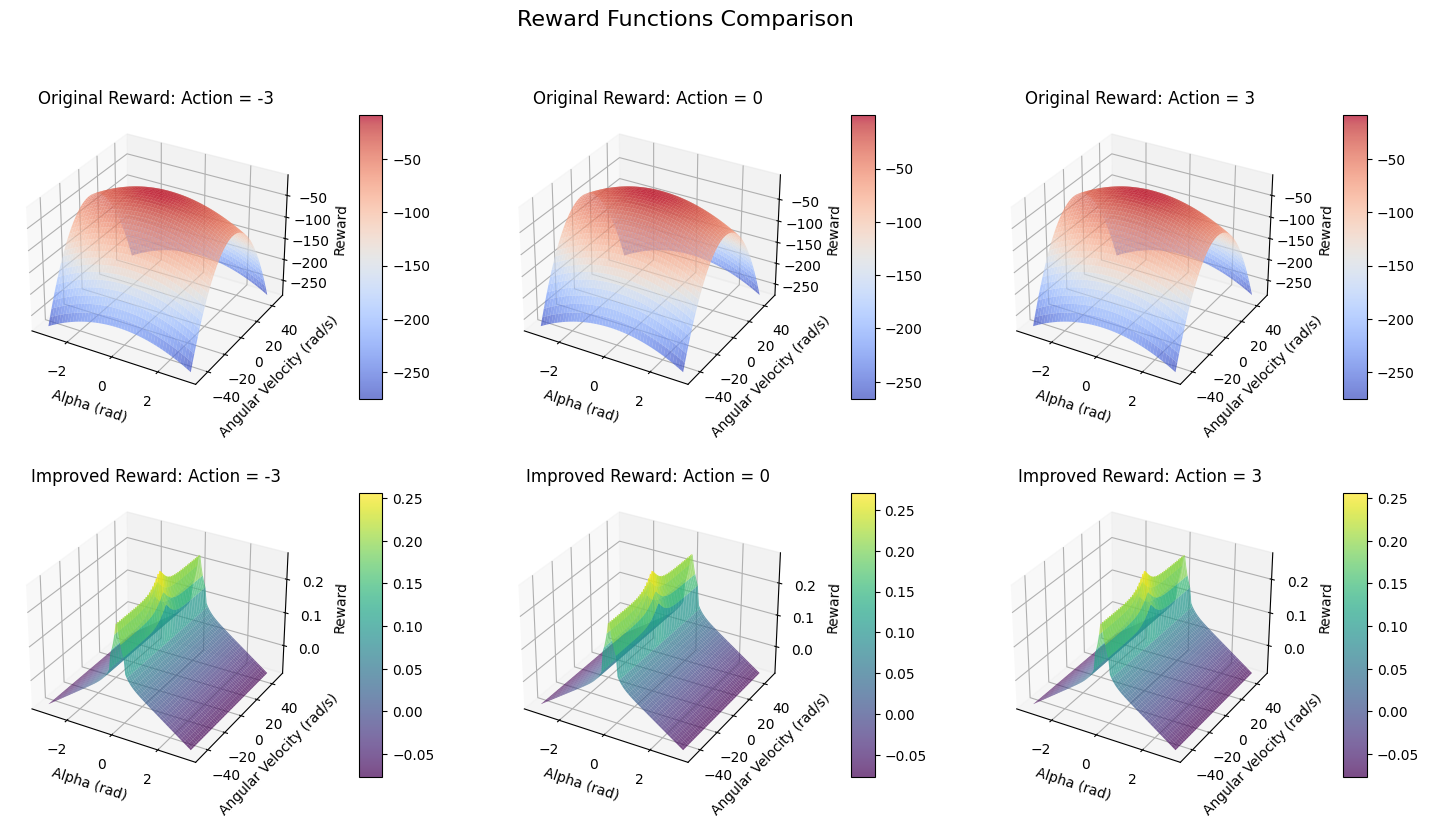
\includegraphics[width=1\textwidth]{images/pendulum_reward_compare.png}
    \caption{改进奖励与原始奖励对比}
    \label{fig:compare}
\end{figure}

对应代码为:
\begin{lstlisting}
# envs/pendulum_env.py
# ...
class PendulumEnv(Env):
# ...
    def step(self, action: float) -> tuple:
        # ...
        
        # original reward
        # reward = -5 * np.power(self.alpha, 2) - 0.1 * np.power(self.dot_alpha, 2) - np.power(action, 2)
        # reward *= 1e-2

        # improved reward
        upright_angle = -np.abs(self.alpha) + np.pi / 2
        reward = 0.05 * (
            upright_angle + 0.001 * np.exp(upright_angle * 5)
        )  # higher value like 0.2 or lower value like 0.001 might be hard for DQN to learn

        if np.abs(np.degrees(self.alpha)) < 20:
            velocity_penalty = 0.05 * (np.tanh(np.abs(self.dot_alpha) * 0.1))
            action_penalty = 0.05 * (np.tanh(np.abs(action) * 0.1))
            reward += 0.1 - velocity_penalty - action_penalty
# ...
\end{lstlisting}

本作业中,将倒立摆环境建模为连续状态空间与离散动作空间。状态包括角度(限制在$[-\pi,\pi)$,弧度制)和角速度(限制在$[-15\pi,15\pi]$,弧度制)。动作为$\{-3,0,3\}$。这部分以及环境参数均与作业要求保持一致。

在训练中,还观察到若在训练前期环境每更新一步智能体就采取动作可能导致局部最优。这可能是因为网络初始参数(以及DQN的初始高$\epsilon$)对应动作期望接近于0,导致无法起摆。为了避免该问题,训练以较高的动作间隔(如环境每10步更新一次动作)开始,逐渐减小到1。

\subsection{冰壶游戏}

冰壶游戏中,控制冰壶在随机初始状态出发,到达并停止在随机目标位置。建立冰壶的离散动力学模型:
\begin{equation}
    \begin{cases}
    \mathbf{D}_t = -0.005 \cdot \|\mathbf{v}_t\| \cdot \mathbf{v}_t \\
    \mathbf{a}_t = \frac{1}{m} \left( \mathbf{F}_t + \mathbf{D}_t \right) \\
    \mathbf{v}_{t+1} = \mathbf{v}_t + \mathbf{a}_t \cdot \Delta t \\
    \mathbf{x}_{t+1} = \mathbf{x}_t + \mathbf{v}_t \cdot \Delta t
    \end{cases}
\end{equation}
其中,$\mathbf{D}_t$为空气阻力,大小为$0.005\|\mathbf{v}_t\|^{2}$,方向为$-\mathbf{v}_t$。$\mathbf{F}_t$为智能体输入的力,$\mathbf{a}_t$为加速度,$\mathbf{v}_t$为速度,$\mathbf{x}_t$为位置。当碰撞墙壁时速度大小变为原来的0.9倍,并发生反弹。对应代码:
\begin{lstlisting}
# envs/curling_env.py
# ...
class CurlingEnv(Env):
# ...
    def _update_speed(self, action: tuple[float, float]) -> None:
        """
        Update the speed of the stone based on the action taken.
        """
        drag = -0.005 * np.linalg.norm(self.current_speed) * np.array(self.current_speed)
        acceleration = (np.array(action) + drag) / self.m
        self.current_speed = tuple(np.array(self.current_speed) + acceleration * self.dt)

    def _update_position(self) -> None:
        """
        Update the position of the stone based on the current speed.
        """
        new_x = self.current_position[0] + self.current_speed[0] * self.dt
        new_y = self.current_position[1] + self.current_speed[1] * self.dt

        # Check for rebound with walls, consider radius of the curling stone
        if new_x - self.r < 0 or new_x + self.r > self.w:
            new_x = max(self.r, min(new_x, self.w - self.r))
            self.current_speed = (
                self.rebound_coefficient * -self.current_speed[0],
                self.rebound_coefficient * self.current_speed[1],
            )
        if new_y - self.r < 0 or new_y + self.r > self.h:
            new_y = max(self.r, min(new_y, self.h - self.r))
            self.current_speed = (
                self.rebound_coefficient * self.current_speed[0],
                self.rebound_coefficient * -self.current_speed[1],
            )

        self.current_position = (new_x, new_y)
# ...
\end{lstlisting}

奖励函数为:
\begin{equation}
    \mathcal{R}(s)=-\|\mathbf{x}-\mathbf{y}\|
\end{equation}
其中$\mathbf{x}$为冰壶所在位置,$\mathbf{y}$为目标位置。

与倒立摆环境类似,将冰壶环境形式化为连续状态空间与离散动作空间。状态空间包括冰壶位置,冰壶速度和目标位置,均为2维向量,共6维状态。动作空间为$\{(5,0),(0,5),(-5,0),(0,-5)\}$即四个方向上的力。

在PPO的训练中,发现若不对奖励和状态进行标准化会导致训练无法收敛,而DQN不存在这样的问题。因此,在PPO训练中,奖励缩放至-1到0,位置缩放至0到1,速度按比例缩放。见下面的代码:
\begin{lstlisting}
# envs/curling_env.py
# ...
class CurlingEnv(Env):
# ...
    def _get_state(self) -> tuple[float, float, float, float, float, float]:
        if not self.normalize:
            # ...
        else:
            return (
                self.current_position[0] / self.w,
                self.current_position[1] / self.h,
                self.current_speed[0] / self.initial_speed_range[1],
                self.current_speed[1] / self.initial_speed_range[1],
                self.target_position[0] / self.w,
                self.target_position[1] / self.h,
            )
# ...
    def _calculate_reward(self) -> float:
        # ...
        distance = np.linalg.norm(np.array(self.current_position) - np.array(self.target_position))
        reward = -distance
        if self.normalize:
            reward /= np.linalg.norm(np.array([self.w, self.h]))  # Normalize reward
        return reward
# ...
\end{lstlisting}

\section{算法}
\label{sec:algo}

\subsection{DQN}
Deep Q-Network (DQN) 结合Q-Learning与深度神经网络,通过经验回放和固定目标网络解决稳定性问题。核心要素为:

\begin{itemize}
    \item 经验回放:存储转移样本$(s_t,a_t,r_t,s_{t+1},d_t)$到缓冲区,随机采样打破相关性
    \item 目标网络:使用独立参数$\theta^-$计算目标值,定期与在线网络$\theta$同步
    \item 损失函数:最小化时序差分误差
\end{itemize}

Q值更新公式:
\begin{equation}
    \label{eq:dqn_target}
    y_t = r_t + \gamma (1 - d_t) \max_{a'} Q_{\theta^-}(s_{t+1}, a')
\end{equation}

损失函数:
\begin{equation}
    \label{eq:dqn_loss}
    \mathcal{L}(\theta) = \mathbb{E}_{(s,a,r,s',d)\sim\mathcal{D}} \left[ \left( Q_\theta(s,a) - y_t \right)^2 \right]
\end{equation}

其中$\gamma$为折扣因子,$\mathcal{D}$为经验回放缓冲区。代码实现为:
\begin{lstlisting}
# agents/dqn.py
# ...
class DQNAgent(Agent):
# ...
    def update(self, buffer: dict) -> dict[str, float]:
        # ...
        # Compute Q-values for current states
        q_values = self.q_network(states).gather(1, action_ids)  # Batch size x 1

        # Compute target Q-values for next states
        with torch.no_grad():
            next_q_values = self.target_network(next_states).max(1)[0].view(-1, 1)  # Batch size x 1

        # Compute target values
        targets = rewards + (1 - dones) * self.gamma * next_q_values

        # Compute loss
        loss = self.loss_fn(q_values, targets)

        # Optimize the Q-network
        self.optimizer.zero_grad()
        loss.backward()
        self.optimizer.step()

        # Update the target network
        self._update_counter += 1
        if self._update_counter % self.target_update_interval == 0:
            self.target_network.load_state_dict(self.q_network.state_dict())
            self.target_network.eval()
# ...
\end{lstlisting}

\subsection{PPO}
Proximal Policy Optimization (PPO) 是一种策略梯度算法,通过限制策略更新幅度保证稳定性。核心特征包括:

\begin{itemize}
    \item 截断(PPO-Clip):限制策略更新幅度
    \item 优势估计(GAE):使用价值函数基线减少方差
    \item 多轮mini-batch更新:提高样本利用率
\end{itemize}

优势函数计算公式为:
\begin{equation}
    \label{eq:gae}
    A_t = \sum_{k=0}^{T-t} (\gamma \lambda)^k \delta_{t+k}
\end{equation}
其中$\delta_t = r_t + \gamma V_\psi(s_{t+1}) - V_\psi(s_t)$为TD残差。

策略目标函数表示为:
\begin{equation}
    \label{eq:ppo_clip}
    \mathcal{L}^{\text{CLIP}}(\phi) = \mathbb{E}_t \left[ \min\left( \frac{\pi_\phi(a_t|s_t)}{\pi_{\phi_{\text{old}}}(a_t|s_t)} A_t, \text{clip}\left( \frac{\pi_\phi(a_t|s_t)}{\pi_{\phi_{\text{old}}}(a_t|s_t)}, 1-\epsilon, 1+\epsilon \right) A_t \right) \right]
\end{equation}

价值函数损失:
\begin{equation}
    \label{eq:value_loss}
    \mathcal{L}^{\text{VF}}(\psi) = \mathbb{E}_t \left[ (V_\psi(s_t) - R_t)^2 \right]
\end{equation}

总损失函数:
\begin{equation}
    \label{eq:ppo_total}
    \mathcal{L}^{\text{Total}} = \mathcal{L}^{\text{CLIP}} - c_1 \mathcal{L}^{\text{VF}} + c_2 \mathcal{H}(\pi_\phi(\cdot|s_t))
\end{equation}

其中$\epsilon$为clip范围,$c_1,c_2$为系数,$\mathcal{H}$为策略熵。价值函数损失由Critic网络优化,其余损失由Actor网络优化。代码为:
\begin{lstlisting}
# agents/ppo.py
# ...
class PPOAgent(Agent):
# ...
    def update(self, buffer: dict) -> dict[str, float]:
        # ...
        # Compute current values
        with torch.no_grad():
            values = self.value_network(states)
            next_values = self.value_network(next_states)

        # Compute advantages and returns
        advantages, returns = self.compute_advantages(rewards, values, next_values, dones)

        # ...
        for _ in range(self.ppo_epochs):
            # Generate random indices for mini-batches
            indices = torch.randperm(states.size(0))

            # Process mini-batches
            for start_idx in range(0, states.size(0), self.mini_batch_size):
                # ...
                # Get current policy distribution
                logits = self.policy_network(batch_states)
                dist = torch.distributions.Categorical(logits=logits)

                # Get current log probs
                batch_new_log_probs = dist.log_prob(batch_actions).unsqueeze(1)

                # Calculate entropy
                entropy = dist.entropy().mean()

                # Calculate ratio between new and old policies
                ratio = torch.exp(batch_new_log_probs - batch_old_log_probs)

                # Calculate surrogate losses
                surr1 = ratio * batch_advantages
                surr2 = torch.clamp(ratio, 1.0 - self.clip_ratio, 1.0 + self.clip_ratio) * batch_advantages
                policy_loss = -torch.min(surr1, surr2).mean()

                # Calculate value loss
                value_pred = self.value_network(batch_states)
                value_loss = F.mse_loss(value_pred, batch_returns)

                # Calculate total loss
                # loss = policy_loss + self.value_coef * value_loss - self.entropy_coef * entropy
                actor_loss = policy_loss - self.entropy_coef * entropy
                critic_loss = self.value_coef * value_loss

                # Update policy network
                self.policy_optimizer.zero_grad()
                actor_loss.backward()
                self.policy_optimizer.step()

                # Update value network
                self.value_optimizer.zero_grad()
                critic_loss.backward()
                self.value_optimizer.step()
# ...
\end{lstlisting}

\section{实验}
\label{sec:experienment}
两个实验中,算法对应的网络均使用MLP,包含两个128维隐藏层。训练时种子固定,以便复现与结果对比。每个实验都尝试过几十个超参数组合,作业中仅呈现结果最佳的数据。在大量实验中发现:两个算法对超参数都非常敏感,尤其是PPO作为on-policy算法在多轮训练中若数据方差较大,可能导致无法收敛。因此,在实验中PPO的回合数要求远高于DQN,且每次更新前需要采集大量数据。

\subsection{倒立摆实验}

实验限制环境为最多500步,DQN的初始动作间隔为20步,PPO为10步。奖励的折扣因子均为0.98。DQN的初始$\epsilon$为0.9,逐渐减少为0.0001。为加速训练,DQN每10步训练一次,每次采样4096个样本,目标网络每20次训练进行一次更新。PPO每4096条样本进行一次训练,每次训练在总样本上迭代12轮,mini-batch大小为64。DQN共训练200回合(episode),PPO训练600回合。

\begin{figure}[htbp!]
    \centering
    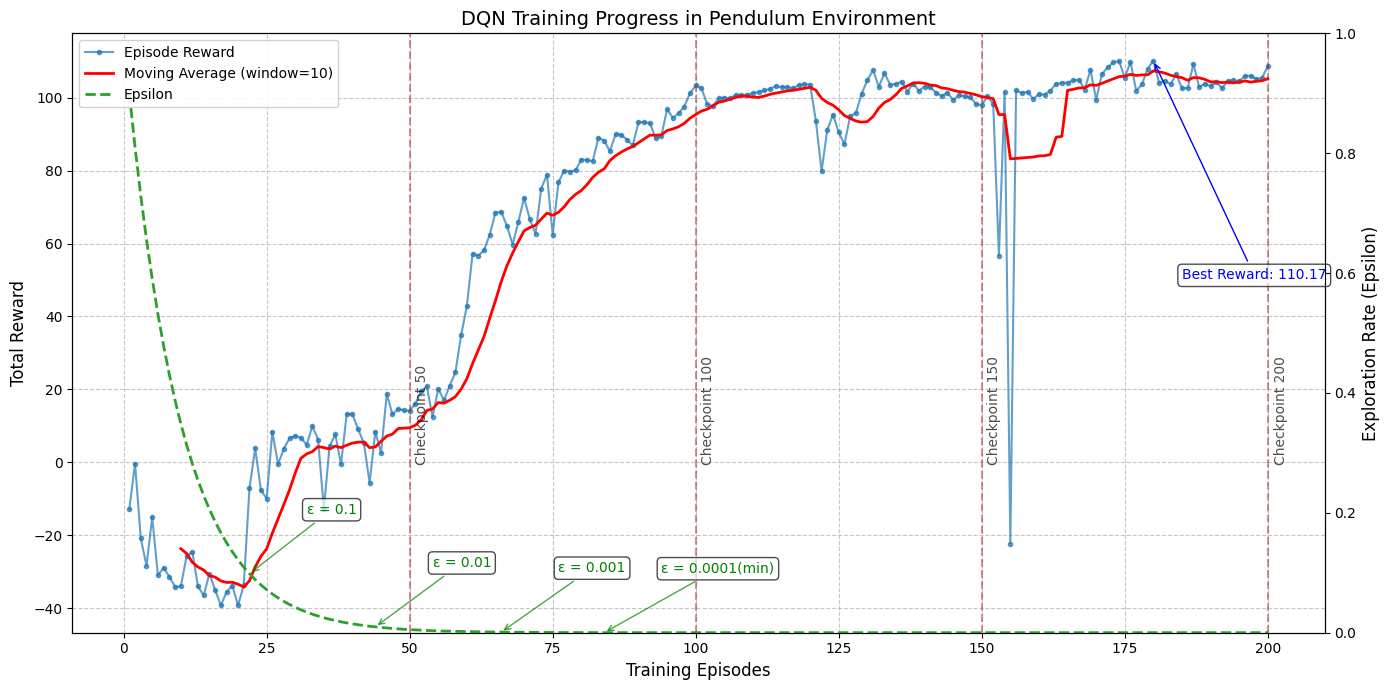
\includegraphics[width=1\textwidth]{images/pendulum_dqn_train.png}
    \caption{DQN的倒立摆训练曲线}
    \label{fig:pendulum_dqn_train}
\end{figure}
\begin{figure}[htbp!]
    \centering
    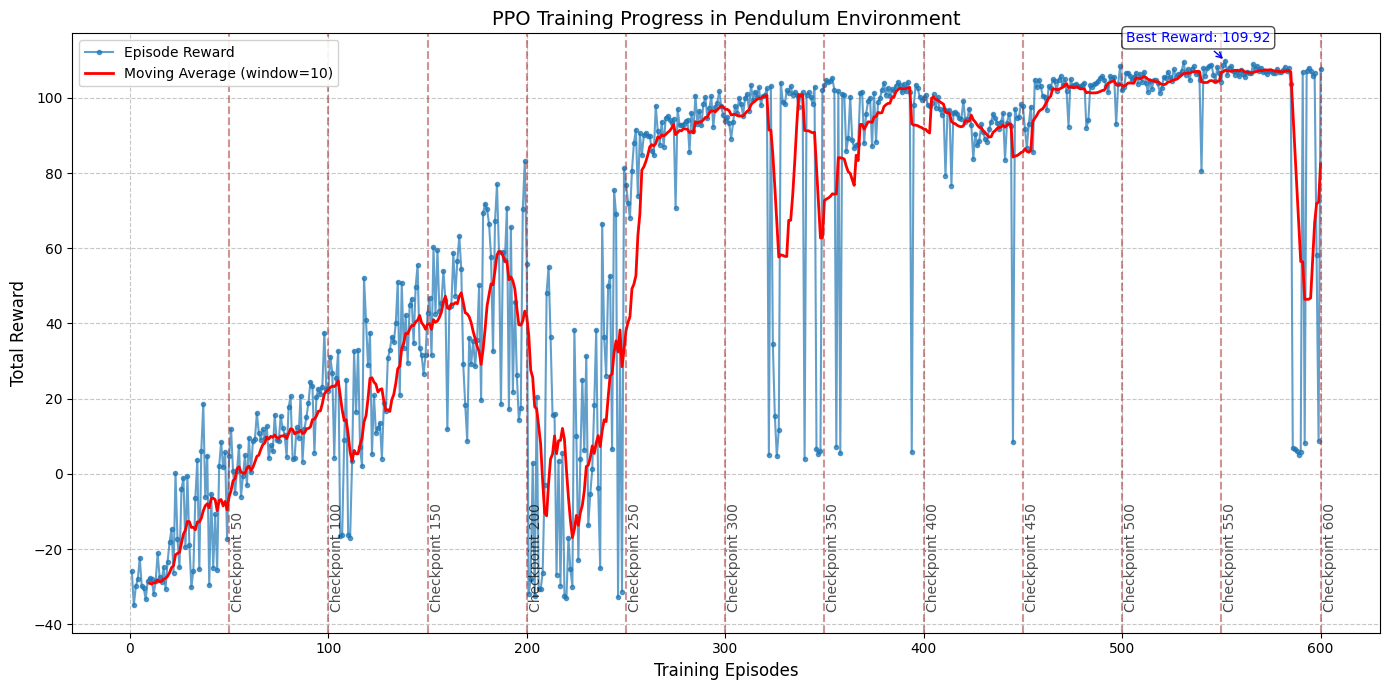
\includegraphics[width=1\textwidth]{images/pendulum_ppo_train.png}
    \caption{PPO的倒立摆训练曲线}
    \label{fig:pendulum_ppo_train}
\end{figure}

训练过程的奖励曲线如图\ref{fig:pendulum_dqn_train}和\ref{fig:pendulum_ppo_train}所示。注意到PPO的奖励波动较大,这可能是因为策略的随机性导致的。在评估时,DQN和PPO均采用确定性策略,采用最终的模型检查点。评估环境为2000步,并在中间引入顺时针和逆时针的短暂扰动,测试策略的抗扰动能力。额外的,设计了一个PID基线作为对比。

\begin{figure}[htbp!]
    \centering
    \begin{subfigure}[b]{0.49\textwidth}
        \centering
        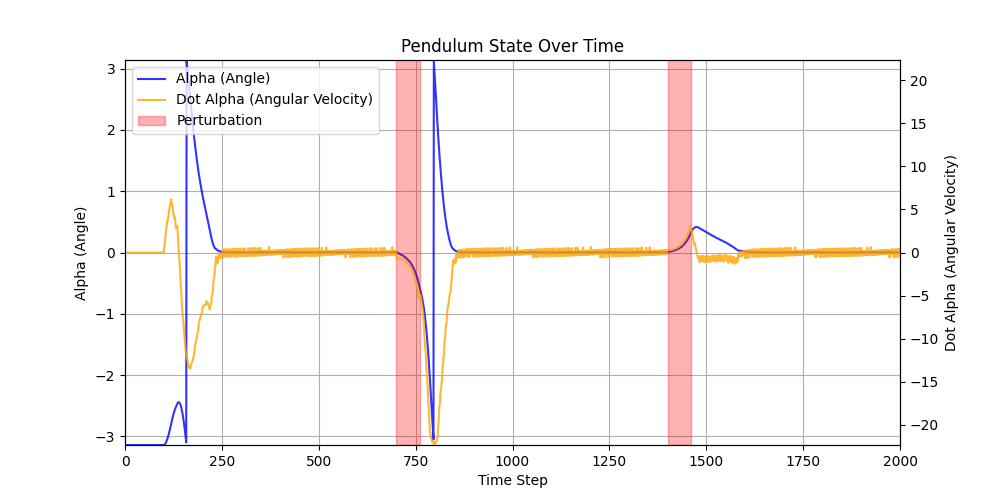
\includegraphics[width=\textwidth]{images/pendulum_dqn_eval.png}
        \caption{DQN的倒立摆评估曲线}
        \label{fig:pendulum_dqn_eval}
    \end{subfigure}
    \hfill
    \begin{subfigure}[b]{0.49\textwidth}
        \centering
        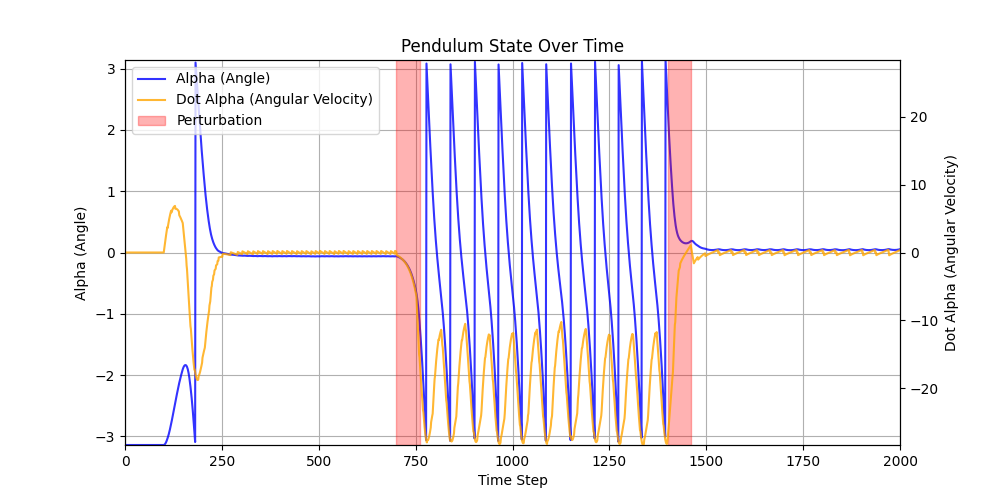
\includegraphics[width=\textwidth]{images/pendulum_ppo_eval.png}
        \caption{PPO的倒立摆评估曲线}
        \label{fig:pendulum_ppo_eval}
    \end{subfigure}
    
    \vspace{0.5cm} % 上下两行之间的垂直间距
    
    \begin{subfigure}[b]{0.49\textwidth}
        \centering
        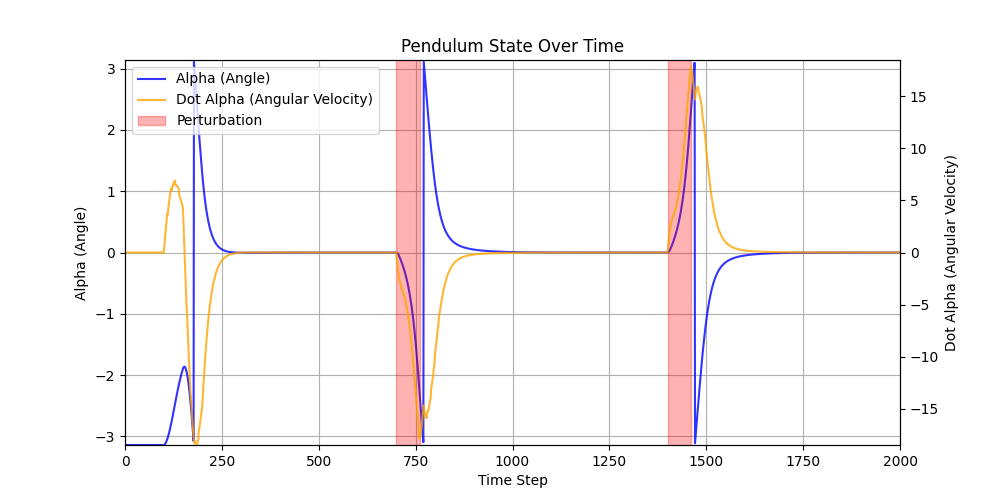
\includegraphics[width=\textwidth]{images/pendulum_pid_eval.png}
        \caption{PID的倒立摆评估曲线}
        \label{fig:pendulum_pid_eval}
    \end{subfigure}
    \caption{三种算法的倒立摆性能比较}
    \label{fig:pendulum_all_eval}
\end{figure}

三者的评估状态曲线见图\ref{fig:pendulum_dqn_eval},\ref{fig:pendulum_ppo_eval}和\ref{fig:pendulum_pid_eval}。因角度限制,图中的锯齿状曲线表示倒立摆旋转一周。注意到三者都能较好的稳定在最高点,但抗扰动能力不同。DQN在第一个扰动下旋转一圈后稳定,在第二个扰动下迅速回正。PPO在第一个扰动下无法自行重新收敛,在第二个反向扰动作用下回到最高点。PID在两个扰动下均旋转一圈后稳定。尽管PPO的表现最差,但在训练时,智能体并没有扰动经验,且学习的轨迹较为固定,难以优化经验较少的状态空间;DQN较好的表现可能具有随机性,在其它参数或随机数种子下也有概率像PPO一样扰动后无法稳定。PID的效果最佳,相比于DQN和PPO,其稳定时角度误差几乎为0,且角速度也极小。但需要指出的是,PID无法自行起摆,而是由程序控制;且PID工作在连续动作空间,动作精度更高。更详细的对比见\colorbox{gray!20}{\texttt{visualization/pendulum}}下的视频。



\subsection{冰壶实验}

\begin{figure}[htbp!]
    \centering
    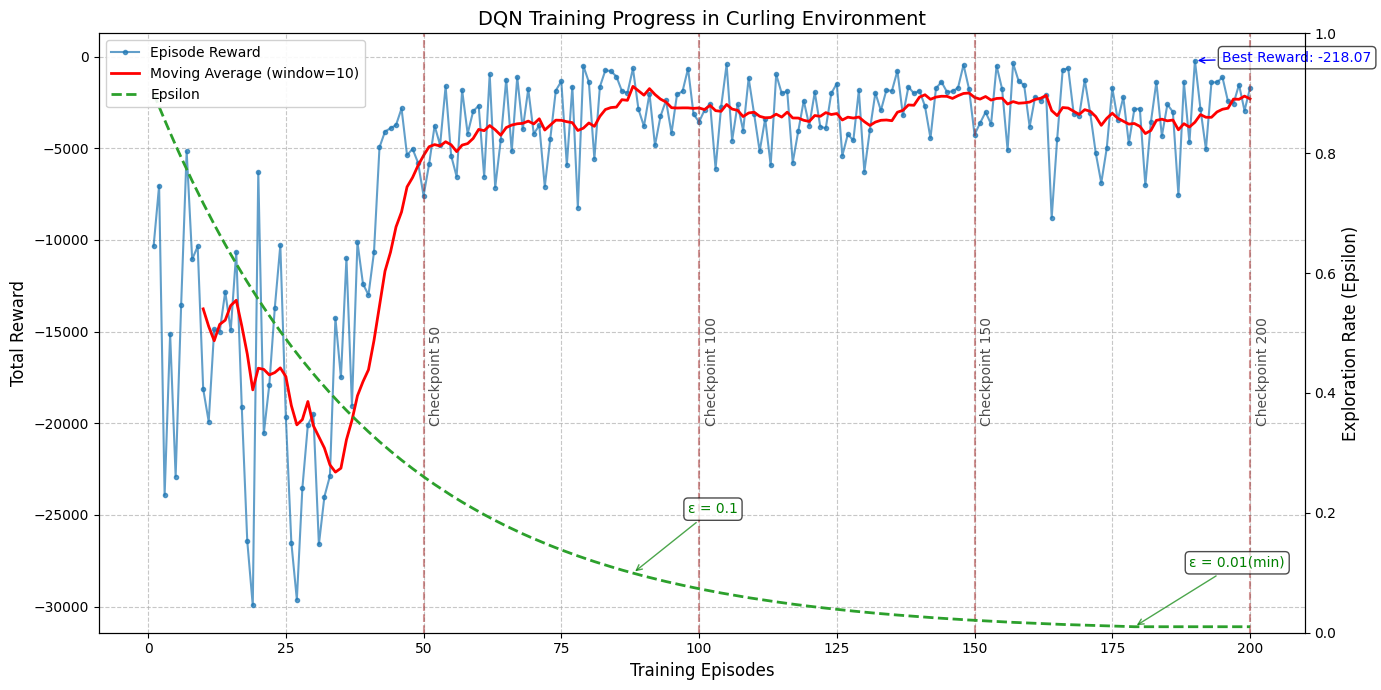
\includegraphics[width=1\textwidth]{images/curling_dqn_train.png}
    \caption{DQN的冰壶游戏训练曲线}
    \label{fig:curling_dqn_train}
\end{figure}
\begin{figure}[htbp!]
    \centering
    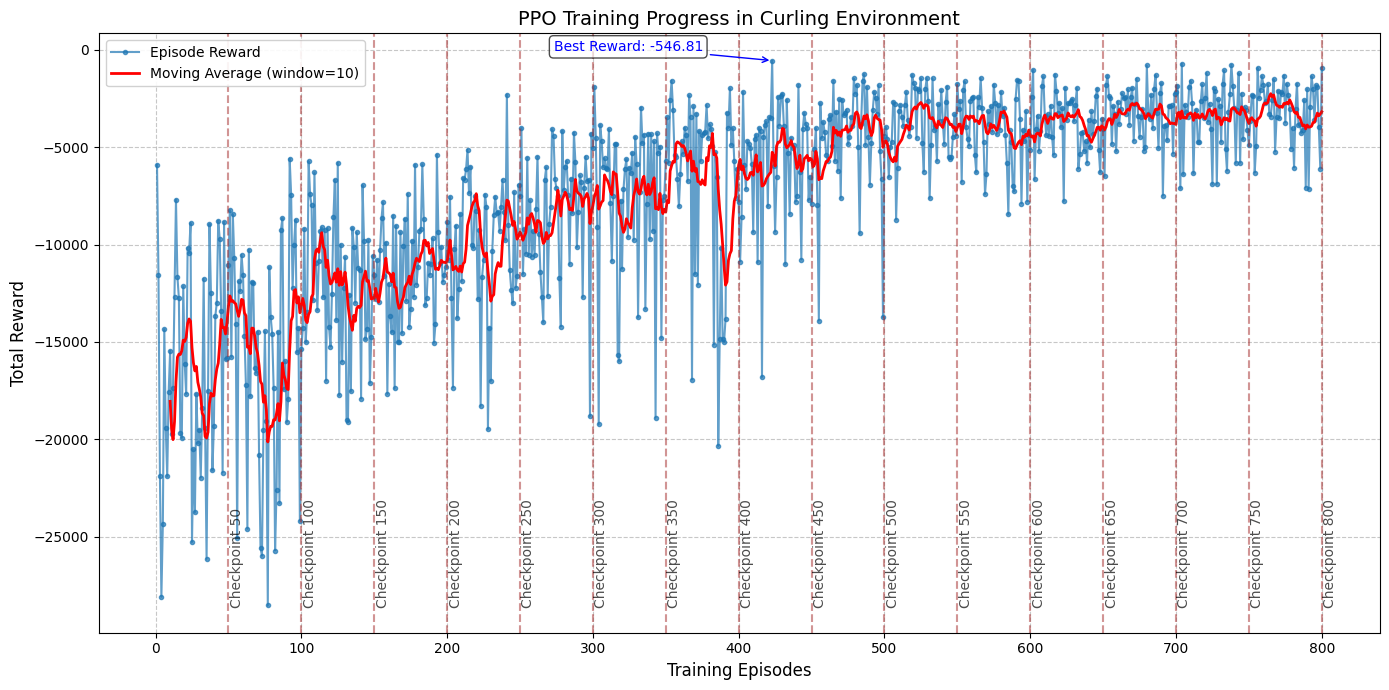
\includegraphics[width=1\textwidth]{images/curling_ppo_train.png}
    \caption{PPO的冰壶游戏训练曲线}
    \label{fig:curling_ppo_train}
\end{figure}

冰壶游戏中每回合限制30秒,即3000步,决策300步。奖励折扣因子为1。DQN的$\epsilon$设置为初始0.9,衰减至0.01,每步都进行在线网络更新,每500步进行目标网络更新,每次采样4096个样本。PPO每8192条样本进行一次训练,每次训练在总样本上迭代10轮,mini-batch大小为256。DQN共训练200个回合,PPO训练800个回合。

训练过程的奖励曲线如图\ref{fig:curling_dqn_train}和\ref{fig:curling_ppo_train}所示。DQN在大约50回合收敛到较优策略,而PPO在大约400回合收敛到较优策略。在DQN训练时,采用了一个较大的目标网络更新步数(500),原因是较小值可能被不同轨迹的方差影响,让网络损失无法收敛。类似的,PPO也需要收集大量的样本(至少2048条以上,即7回合以上)才能保证训练的稳定。

评估过程缩短至15秒,固定随机种子生成5个不同初始状态的环境,得到的距离随时间步的曲线如图\ref{fig:curling_dqn_eval}和\ref{fig:curling_ppo_eval}所示。二者在离目标较远时,均能输出合适动作快速靠近;但是在接近目标后的动作随机性提升,不能实现完全与目标重合,且在两个评估曲线中均出现了先接近后远离的情况。原因可能在于离目标较近时奖励函数变化较小,或者动作仍需进一步增加离散精度,此处没有深入探究。此外,两个模型都没有学习到利用场地反弹接近目标,仅学会让速度矢量指向目标。

\begin{figure}[htbp!]
    \centering
    \begin{subfigure}[b]{0.49\textwidth}
        \centering
        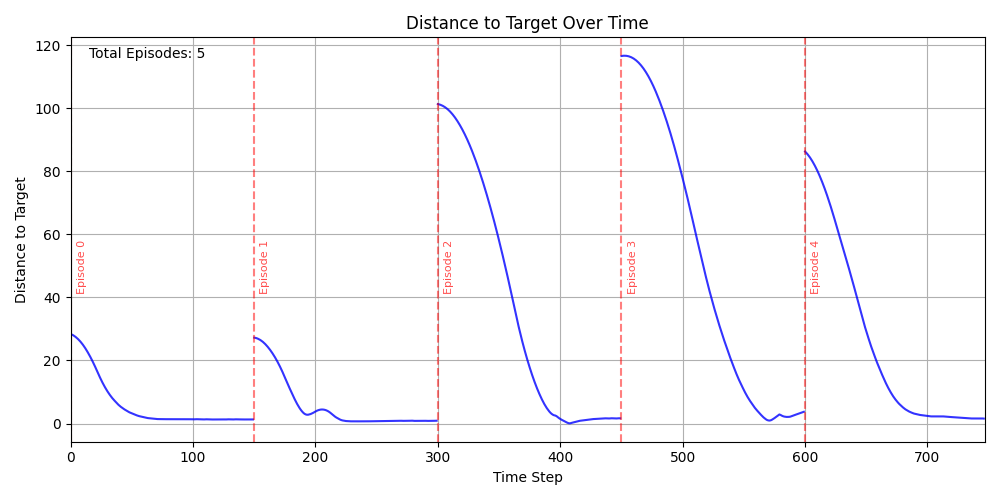
\includegraphics[width=\textwidth]{images/curling_dqn_eval.png}
        \caption{DQN的冰壶游戏评估曲线}
        \label{fig:curling_dqn_eval}
    \end{subfigure}
    \hfill
    \begin{subfigure}[b]{0.49\textwidth}
        \centering
        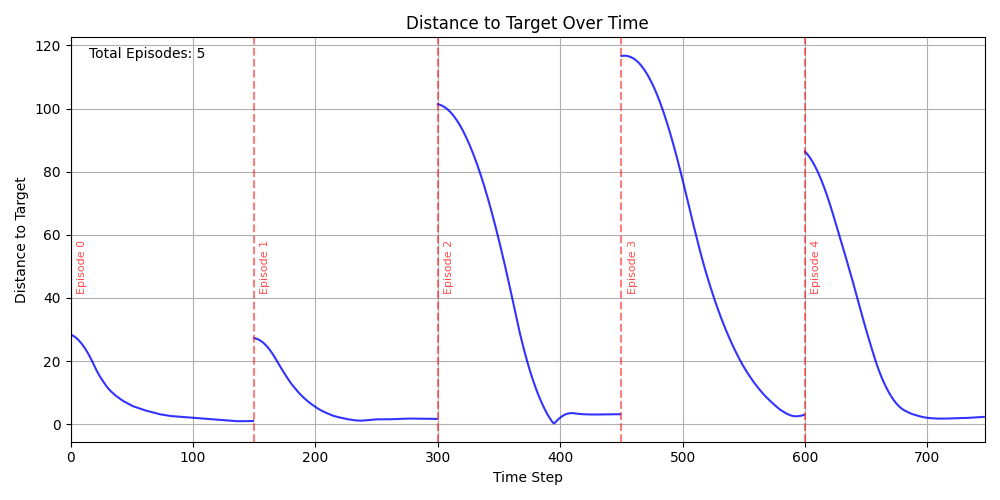
\includegraphics[width=\textwidth]{images/curling_ppo_eval.png}
        \caption{PPO的冰壶游戏评估曲线}
        \label{fig:curling_ppo_eval}
    \end{subfigure}
    \caption{两种算法的冰壶游戏性能比较}
    \label{fig:curling_all_eval}
\end{figure}

\section{总结}
\label{sec:conclusion}
本作业在倒立摆和冰壶游戏两个环境中分别实现了DQN和PPO两种强化学习算法,训练并评估了连续状态空间与离散动作空间的智能体。结果表明,环境的奖励设计与状态的标准化在模型训练中具有重要影响;DQN为代表的off-policy算法比PPO代表的on-policy算法对数据需求量更少;在本作业的实验设计下,PPO比DQN对超参数更敏感,且性能略低于DQN。

% \newpage
% \printbibliography

\end{document}
